\documentclass[12pt]{report}
    
%%%%%%%%%%%%
% Packages %
%%%%%%%%%%%%

\usepackage[english]{babel}
\usepackage[noheader]{packages/sleek}
\usepackage{packages/sleek-title}
\usepackage{packages/sleek-theorems}
\usepackage{packages/sleek-listings}
\usepackage{complexity}
\usepackage{tikz}
\usepackage{algpseudocode}
\usepackage{multirow}
\usepackage{hyperref}
\usepackage{amsthm}
\usepackage[ruled, linesnumbered, noend]{algorithm2e}
\usetikzlibrary{arrows,automata}

%%%%%%%%%%%%%%
% Title-page %
%%%%%%%%%%%%%%

\hypersetup{urlcolor=red}
\urlstyle{same}
\graphicspath{ {./images/} }
\everymath{\displaystyle}
\logo{title.png}
\institute{Habib University}
\faculty{CS 412: Algorithms}
\title{Travelling Salesman Problem}
\subtitle{Implementations and Analysis of Various Solutions}
\author{\textit{Authors}\\
            Ali Hamza \\
            Ali Taher \\
            Muhammad Usaid \\
            Syed Anus}
\date{\today}

%%%%%%%%%%%%%%%%
% Bibliography %
%%%%%%%%%%%%%%%%

\addbibresource{./resources/bib/references.bib}

%%%%%%%%%%
% Others %
%%%%%%%%%%

\lstdefinestyle{latex}{
    language=TeX,
    style=default,
    %%%%%
    commentstyle=\ForestGreen,
    keywordstyle=\TrueBlue,
    stringstyle=\VeronicaPurple,
    emphstyle=\TrueBlue,
    %%%%%
    emph={LaTeX, usepackage, textit, textbf, textsc}
}

\FrameTBStyle{latex}

\def\tbs{\textbackslash}

%%%%%%%%%%%%
% Document %
%%%%%%%%%%%%

\begin{document}
    \maketitle
    \romantableofcontents

\chapter{Introduction}
The travelling salesman problem has a long history of being a problem of interest in the field of algorithms. It has garnered much attention and there has been a lot of work that has been done on it. In this project we will set out to establish the details of this problem and why it is so tough. We will then investigate 4 algorithms that have become well known in being useful for solving this problem. One of them produces an exact solution and the rest use approximation techniques. We will be using theory and implementation to test the run times of this problem and will then present our research in an appropriate format.\par
\textbf{Github:} \url{https://github.com/hurryingauto3/CS412-Algorithms-Final-Project}\par
\textbf{Implementation Notebook:} \url{https://tinyurl.com/yxdyvc6p}
\chapter{Design Techniques}
  \section{Exact Solution}
  
\subsection{1. Held-Karp Algorithm}
The naive exact solution of the travelling salesman problem requires that that each Hamiltonian cycle is travelled and the minimum path of those cycles is found. However, this is an extremely large problem as there will be $O(n!)$ cycles for a complete graph of size $n$. The dynamic programming approach called the Held-Karp algorithm reduces this time complexity to $O(n^22^n)$. It does so by dividing the problem into sub problems.  A very simple method is to visualize this idea using a tree.
  Let us begin this explanation, without loss of generality, with a complete graph, $K_4,$ that does not contain loops. 

\begin{center}
  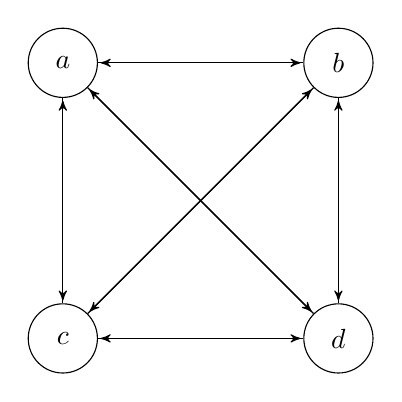
\begin{tikzpicture}[->,>=stealth',shorten >=1pt,auto,node distance=3.5cm,scale = 1,transform shape]

    \node[state] (a) [] {$a$};
    \node[state] (b) [right of=a] {$b$};
    \node[state] (c) [below of=a] {$c$};
    \node[state] (d) [below of=b] {$d$};

    \path (a) edge              node {} (b)
          (b) edge              node {} (a)
          (a) edge              node {} (c)
          (c) edge              node {} (a)
          (a) edge              node {} (d)
          (d) edge              node {} (a)
          (b) edge              node {} (c)
          (c) edge              node {} (b)
          (b) edge              node {} (d)
          (d) edge              node {} (b)
          (c) edge              node {} (d)
          (d) edge              node {} (c);

  \end{tikzpicture}
\end{center}

Starting from vertex \textit{a}, or any vertex to maintain generality, we can build a decision tree that traverses each path, this represents the the power set of the graph
  \begin{center}
      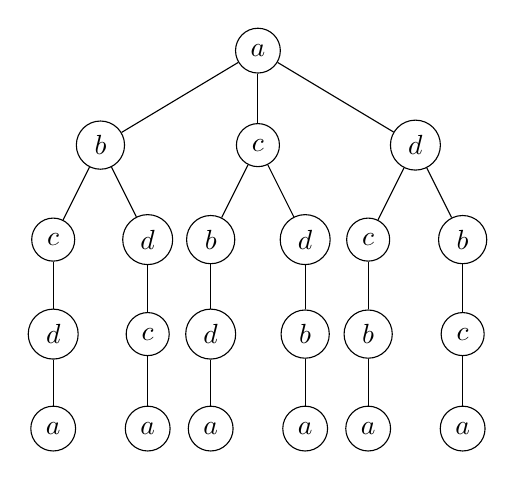
\begin{tikzpicture}[sibling distance=10em,
    every node/.style = {shape=circle, rounded corners,
      draw, align=center,
      top color=white, bottom color=white!5}, scale=0.8]
      \tikzstyle{level 1}=[sibling distance=25mm] 
      \tikzstyle{level 2}=[sibling distance=15mm] 
      \tikzstyle{level 3}=[sibling distance=10mm] 
      
    \node {$a$}
      child { node {$b$} 
          child {node {$c$}
          child {node {$d$}
          child {node {$a$}}}}
          child {node {$d$}
          child {node {$c$}
          child {node {$a$}}}}}
      child { node {$c$} 
          child {node {$b$}
          child {node {$d$}
          child {node {$a$}}}}
          child {node {$d$}
          child {node {$b$}
          child {node {$a$}}}}}
      child { node {$d$} 
          child {node {$c$}
          child {node {$b$}
          child {node {$a$}}}}
          child {node {$b$}
          child {node {$c$}
          child {node {$a$}}}}};
  \end{tikzpicture}
  \end{center}
The idea behind the exhaustive, brute-force approach is to traverse each path in the tree and then decide, this creates a very large problem to solve. The idea behind the dynamic approach is to start from the level 4 of the tree, which means we are now at the last vertex in the path and the next vertex from that completes the cycle and takes us back to the source node. This forms the smallest sub problem in the dynamic program. The next step would be to go a level higher in the tree, which means we will now check the path length and determine whether we are reaching the source node from vertex $v$ and, we are reaching reaching vertex, $v$, from vertex, $u$ s.t. $u,v \in V$ where $V$ is the set of all vertices. We will keep doing this, and at each level we will decide the minimum path length of between n paths that are emerging from one vertex. This is done until the source node of the tree is reached, resulting in the minimum path. The dynamic algorithm can be generalised as a cost function, $g$, as follows:
$$g(i, S) = min_{k\in S} \bigg\{c_{ik} + g(k, S-\{k\})\bigg\}$$
s.t. $i$ is the source vertex, $S$ is the set of all vertices, $c_{ik}$ is the cost of going from some vertex $i$ to $k$. 

\begin{algorithm*}
  \KwIn{A weighted complete graph $G$ and number of nodes $n$}
  \KwOut{An exact optimal Hamiltonian path}
  \For{ k := 2 to n}{
    C({k}, k) := $d_{1,k}$} 
    \For{s := 2 to n $-$ 1 d}{
        \ForEach{\upshape S $\subseteq \lbrace 2,\dots, n \rbrace$, |S| = s}{
            \ForEach{k $\in$ S}{$C(S,k) \leftarrow \min_{m \neq k, m \in S} [C(S\textbackslash \{k\}, m) + d_{m,k}] $}
        }
    }
    opt $\leftarrow \min_{k \neq 1} [C(\{2,3,\dots, n\}, k) + d_{k,1}]$ \\  
  \Return{\upshape opt}
\caption{\textsc{Held Karp Algorithm}}
\end{algorithm*}


\section{Approximate Solutions}
\subsection {Nearest Neighbour Algorithm}
    Nearest Neighbor is one of the approximate solutions to the problem of TSP that finds the cost of travelling from a point and returning back to the original point. To describe the problem in other words, a salesman starts from a city and visits the nearest unvisited city until they have been visited and returns back to the starting city. The algorithm is easy to implement but it does miss shorter paths which does not make it optimal and hence, an approximation.
    The algorithm is as follows: 
    \begin{enumerate}
        \item Choose any starting vertex.
        \item Whenever you reach any vertex, look at the weights of all the edges that lead to vertices you haven’t visited yet. Choose the one that has the least weight.
        \item Repeat step 2 until you’ve reached the last vertex. Else go back to the starting point. 
    \end{enumerate}
        The algorithm is only an approximation but it can be improved by repeating the process and starting from a different vertex each time. This does not mean that the algorithm will give an accurate answer but the chances to get a close to an accurate answer may improve. This is because at each iteration, it only considers the least cost edge whereas it is possible that there could be a path that could have an overall cost that could be less.   
  \subsection {Pairwise Exchange Algorithm}
    First proposed in 1958 by G A Croes, it is a local search algorithm that iteratively optimizes an arbitrary path. The algorithm works by iterating over all possible combinations of two edges that do not share common vertices and replacing them with another edge in a manner such that the total weight of the new edges is less than the total weight of the deleted edges.
    Take the following two edges $u$ and $v$ and let their weights be $w_{1}$ and $w_{2}$:
  \begin{center}
    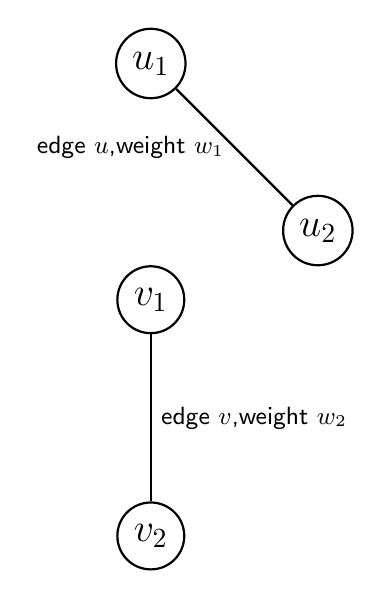
\begin{tikzpicture}[auto, node distance=3cm, every loop/.style={},thick,main node/.style={circle,draw,font=\sffamily\Large\bfseries}]

      \node[main node] (1) {$u_{1}$};
      \node[main node] (2) [below of=1] {$v_{1}$};
      \node[main node] (3) [below of=2] {$v_{2}$};
      \node[main node] (4) [below right of=1] {$u_{2}$};
      
    
      \path[every node/.style={font=\sffamily\small}]
        (1) edge node [left] {edge $u$,weight $w_1$} (4)
    
        (3) edge node [right] {edge $v$,weight $w_2$} (2);
        
    \end{tikzpicture}
  \end{center}
    
    Pairwise exchange will select these two edges and replace them with edges such that the new edges are $uv_{1}$ and $uv_{2}$:
    \begin{center}
    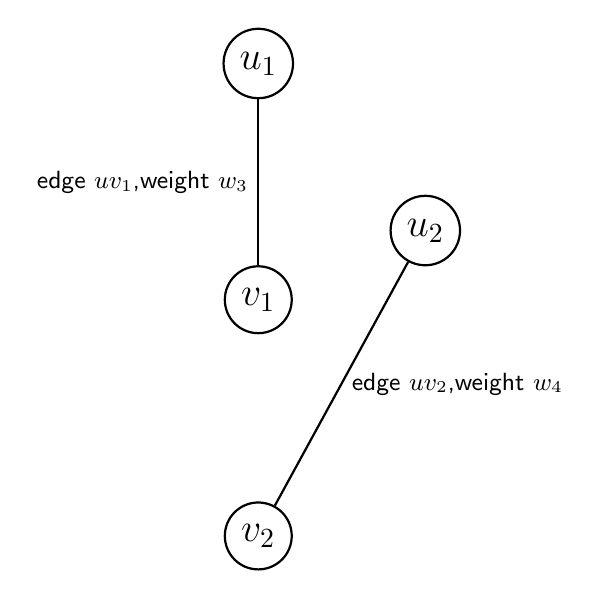
\begin{tikzpicture}[auto, node distance=3cm, every loop/.style={},thick,main node/.style={circle,draw,font=\sffamily\Large\bfseries}]

      \node[main node] (1) {$u_{1}$};
      \node[main node] (2) [below of=1] {$v_{1}$};
      \node[main node] (3) [below of=2] {$v_{2}$};
      \node[main node] (4) [below right of=1] {$u_{2}$};
      
    
      \path[every node/.style={font=\sffamily\small}]
        (1) edge node [left] {edge $uv_{1}$,weight $w_3$} (2)
    
        (3) edge node [right] {edge $uv_{2}$,weight $w_4$} (4);
    
    
        
    \end{tikzpicture}
    \end{center}
    
    The following condition is checked, every time an edge exchange is done:
    
    \[w_{3}+w_{4} - (w_{1} +w_{2})<0\]
    
    The sum of weights of the two new edges and the deleted edges is subtracted to see if there has been a decrease or not. If replacing the edges brings about a decrease in the total weight, then the replaced edges are preserved. Otherwise, the old edges are kept and some other combination of edges are tested for replacement. The algorithm below states the exact steps that we need to make:\\
    
    \begin{algorithm*}
        \KwIn{A weighted complete graph $G$}
        \KwOut{An optimized Hamiltonian path $best_p$}
        Initialize an arbitrary path p \\
        $best_p$=p \\
        While $best_p$ improves: \\
        for $i$ in range(1,length($p.vertices$)-2): \\
        \quad for $j$ in range(i+1,length($p.vertices$)):\\
        \qquad if best($u_{1}$,$v_{1}$)+best($u_{2}$,$v_{2}$)$-$(best($u_{1}$,$u_{2}$)+best($v_{1}$,$v_{2}$)) $<$ 0:\\
        swap edges from $u$,$v$ to $uv_{1}$ and $uv_{2}$\\
    \Return{\upshape the hamiltonian path $best_p$}
    \caption{\textsc{Pairwise Exchange Method}}
    \end{algorithm*}        
    
    Each time the algorithm runs, it checks for each possible edge exchange in a given Hamiltonian path and seeks to decrease the total weight of the path. Hence, each time the algorithm runs, a new path is produced whose total weight may be further minimized. Although, a termination condition may be added to let the outer loop run for a specified number of sequences before giving out the result in order to avoid having to search across all possible \textit{n!} paths.

    \subsection{Christofides–Serdyukov Algorithm}
    The Christofides–Serdyukov algorithm is another approximation algorithm, that gives a solution that is relatively close to the optimal TSP tour. First, we will take a look at a simpler approximation algorithm that results in an approximation ratio of 2.

    \begin{algorithm*}
      \KwIn{A weighted complete graph $G$ and a root vertex $v$}
      \KwOut{A hamiltonian cycle $H$.}
      compute a minimum spanning tree $T$ for $G$ using \textsc{MST-PRIM}($G, v$) \\
      let $H$ be the list of vertices, ordered according to when they are first visited in a
      preorder tree walk of $T$ \\
      \Return{\upshape the hamiltonian cycle $H$}
  \caption{\textsc{approx-tsp-tour}}
  \end{algorithm*}
    
  This algorithm relies on the assumption that the weights of the edges of the graph conform to the triangle inequality and that the graph is complete.
  Let $c(u,v)$ be the weight of an edge. Then, \[c(u,w) \leq c(u,v) + c(v, w) \]
  In simpler words, removing an intermediate stop would never increase the cost. If the edges do not conform to the triangle inequality, then a polynomial-time approximation
  with a constant approximation ratio does not exist, unless $\mathbf{P = NP}$. The proof of this
  is outside the scope of this paper. This version of the TSP is also called a metric TSP since 
  the edge weights form a metric space.   
  \par Let's look at a short proof that \textsc{approx-tsp-tour} is a poly-time 2- approximation algorithm. 
  \par
  \begin{proof}
  

    Let $H^*$ denote the optimal TSP tour for a set of vertices. We can obtain a spanning tree $T$ by eliminating an edge from 
    $H^*$. This provides a lower bound for cost of $H*$. 
    \[c(T) \leq c(H^*)\] A full walk $W$ of $T$ would visit every edge of $T$ twice, which means   
    \[c(W) = 2\cdot c(T) \implies c(W) \leq 2\cdot c(H^*)\]
  Since, the triangle inequality is being obeyed, we can remove repeated visits in $W$ with a guarantee that 
  the cost will not increase.
  Let $H$ be the cycle corresponding to a pre-order walk in $T$. This hamiltonian cycle is the cycle that is computed by 
  \textsc{approx-tsp-tour}. Since $H$ is obtained by deleting vertices from $W$,
  \[c(H) \leq c(W)\]
  This implies that, \[c(H) \leq 2\cdot c(H^*)\] which completes the proof. 
  \par
        \end{proof}
    \newpage
  {{\textbf{An Improved Algorithm:}}}  \par
  
  This algorithm can be improved by adding a few more graph operations that can further optimize our solution.
  The improved algorithm by Christofides relies on the same assumptions (triangle inequality and complete graph). 
  However, it utilizes other graph properties to improve the approximation ratio. These facts/properties are:
  \begin{enumerate}
    \item[1] The number of vertices with odd degree in a graph is always even, according to the handshaking lemma. 
    \item[2] A graph that has all vertices with even degree will have an Eulerian tour. 
    \item[3] Given a complete weighted graph with an even number of vertices, a minimal weight perfect matching can be found in polynomial 
     time. Specifically, it can be computed in $O(|E||V|^2)$  using the Blossom algorithm by Jack Edmonds.
  \end{enumerate} 
  
  
  \begin{algorithm*}
  
    \KwIn{A weighted, complete graph $G$, and a root vertex $v$.}
    \KwOut{A circuit $\Gamma$}
    compute a minimum spanning tree $T$ for $G$ using \textsc{mst-prim}($G, v$) \\
    let $O$ be the set of vertices with odd degree in $T$ \\
    find an induced subgraph $G'$ given by vertices in $O$ \\
    find a minimum-weight perfect matching $M$ in $G'$ \\
    combine the edges of $M$ and $T$ to form an Eulerian multigraph $M^*$ \\
    find an Eulerian circuit $\Gamma$ in $M^*$ \\
    make $\Gamma$ a Hamiltonian cycle by skipping repeated vertices \\
    \Return{\upshape the Hamiltonian cycle $H$}
    \caption{\textsc{Christofides-Seryukov}}
\end{algorithm*}

\newpage
\chapter{Theoretical Run time Analysis}
\subsection{Held Karp Algorithm}
The algorithm, even though it belongs to \textbf{EXPTIME} and \textbf{EXSPACE}, provides a great computational speed up whilst maintaining the ability to output the exact optimal Hamiltonian path. The time and space complexities are $O(n^2 2^n)$ and $O(n2^n)$ respectively. The fundamental operations employed in the computation are additions and comparisons. The number of each in the first phase is given by: 
$$\bigg( \sum_{k = 2}^{n-1}k(k-1) \frac{(n-1)!}{k!(n-1-k)!}\bigg) + (n-1) = (n-1)(n-2)2^{n-3} + n-1 = \mathbf{O}(n^22^n)$$
and the number of each in the second phase is given by: 
$$\sum_{k=2}^{n-1}k = \frac{n(n-1)}{2} - 1$$
\subsection{Nearest Neighbor Algorithm }
Talking about the nearest neighbor, we can say that it is not optimal. This is because if we consider the brute-force approach, we get an accurate answer. Brute-force calculates the total cost of each Hamilton circuit and returns the minimum out of them. Hamilton circuit is a circuit where it travels to each vertex only once. As it can be seen that the cost of brute force gives us 23 whereas in nearest neighbor, even if we start from any vertex, we still end up with the cost that is greater than 23. However, nearest neighbor is efficient because it does not require to traverse through all the possible edges instead it uses the least weight whereas brute force calculates all possibilities taking n!. Nearest neighbor is $n^2$ because at each point, we need to find its nearest neighbor so that is n. And computing the distance from one point to all the other is n. So total is $O(n^2)$.

  \subsection{Pairwise Exchange Algorithm}
Each time a while loop runs, it takes a total of $O(n^2)$ times. The while loop in itself will only stop when the total weight of the Hamiltonian path converges to an optimal value. The rate of convergence depends on the initial Hamiltonian path that is provided to the algorithm.

Each successive iteration of while loop produces an updated path with a total weight that is less than the previous path. In principal, the algorithm is doing an exhaustive search through all the possible Hamiltonian paths of a given graph. Every time we get a path, we can iterate over it for optimizion. Hence the total running time is $O(n!)$ since there are $n!$ possible permutations as stated in section 1.1.

Each time a while loop runs, it takes a total $O(n^2)$ times. The while loop in itself will only stop when the total weight of the hamiltonian patn converges to an optimal value. In theory, the while loop does not converge at all. Every time we get a path, we can iterate over all of the possible edge exchanges to optimize the path, so this algorithm is an exhaustive search over all of the possible optimal solutions. Hence, the time complexity is O(n!).
\subsection{Christofides–Serdyukov Algorithm}

\par
  Initially, a minimum spanning tree $T$ is constructed. Then from $T$, we add vertices with odd degree to the set $O$. 
  Then we create a subgraph: $G' = G[O]$, i.e. a subgraph induced by the vertices in $O$. Due to Fact 1, this subgraph has 
  even number of vertices. We then find a minimum weight perfect matching $M$ on $G'$, add this matching to the MST $T$, creating 
  an Eulerian multigraph $M^*$. This multigraph will have all vertices having an even degree. This makes it possible for us 
  to find an Eulerian circuit $\Gamma$ in $M^*$. We then reduce $\Gamma$ to a Hamiltonian circuit using the triangle inequality 
  property to remove repeated vertices. The resulting circuit is our approximate solution to the problem. 
  \par
  This algorithm is a $\frac{3}{2}$-approximation algorithm. Let us look at the proof of this. 
  
  \begin{proof}
  

  \par
    Let $H^*$ be the optimal TSP tour and $c(H^*)$ be its weight. 
    Since $T$ is an MST in $G$, \[c(T) \leq c(H^*)\] 
    Let $R$ be the solution to the TSP problem on subgraph $G'$. This means that $c(R) \leq c(H^*)$. We can partition the minimum weight perfect matching 
    on subgraph $G'$. The cost of these partitions is going to sum to $c(R)$; therefore, the smaller of these two partitions is 
    going to be at most $c(R)/2$. Since $M$ is a minimum weight perfect matching on $G'$, will be at most smaller than the partitions of $R$. 
    Therefore, \[c(M) \leq \frac{c(R)}{2}\]
    And so, \[c(T) + c(M) \leq c(H^*) + \frac{c(R)}{2} \leq \frac{3}{2} \cdot c(H^*)\]
    Because of the triangle inequality, short cuts will lead to a better cost. Therefore, 
    \[c(H) \leq c(T) + c(M) \] where $H$ is the approximate tour returned by the Christofides-Seryukov algorithm. This leads to
    \[c(H) \leq \frac{3}{2} \cdot c(H^*)\]
    which concludes our proof.
      \end{proof}

  \textbf{Analysis:} \par
  \textsc{approx-tsp-tour} is an $O(n)$ algorithm since all operations in this algorithm are linear and if Prim's algorithm is 
  implemented using adjacency lists and binary heaps. Otherwise, Prim's algorithm would be $O(n^2)$ in the 
  case of adjacency matrix and would dominate the runtime of \textsc{approx-tsp-tour} making it $O(n^2)$.
  \par The time complexity of the Christofides–Serdyukov algorithm depends on the most expensive operation in the 
  algorithm - finding a minimum weight perfect matching (line 4). This operation is implemented using the Blossom algorithm, which is $O(n^3)$. All the other 
  processes are linear, which means that this algorithm would be $O(n^3)$, where $n$ is the number of vertices. 
\chapter{Empirical Run time Analysis}
We have implemented these algorithms in Python. The programs are run inside a python notebook on a PC with a 3.4Ghz processor. These run times reflect the effect of all of these factors. However, it is an assumption that the empirical run times will grow with the same pattern over any machines, and any language. However, this is only based on the assumption that the theoretical run times are accurate. We can see that most of the algorithms are running close to the predicted time complexity according to the run time trends observed in their graphs

\subsection{Held-Karp}
Due to the extremly high computational space and time complexity of the Held Karp algorithm it is almost impossible for normal machines to be able to run it on a large numbers of vertices. Even running the algorithm on a graph of 20 vertices requires 419430400 operations and 20971520 space units. Therefore, it was very hard to test this algorithm empirically. The code that was used, was taken from a GitHub repository and despite there being many optimizations present in the code the code did not execute for more than 20 vertices in a reasonable amount of time. This experiment produced the following graph, it really does not tell us much about the trend in the empirical running time of the code as theres is too little information present. However, it is very clear that this algorithm is merely a theoretical feat but of little use in practicality as its space complexity is very high and renders is quite useless.  
\begin{center}
    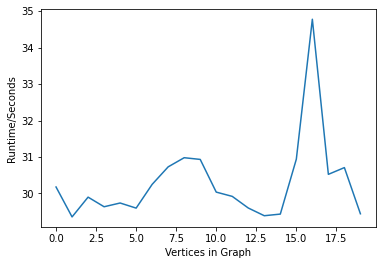
\includegraphics[scale = 0.75]{images/heldkarp.png}
\end{center}

\subsection{Nearest Neighbor}
Talking about the nearest neighbor algorithm, we see from the graph below that it runs extremely fast and is efficient as compared to the brute force algorithm. However, as mentioned earlier nearest neighbor is not optimal as it does not give us the accurate answer. The reason why the algorithm runs so fast is because it does not traverse over every path in the complete graph. However, it only traverses over those nodes which are not visited and have the least weight amongst them that are connected.

\begin{center}
    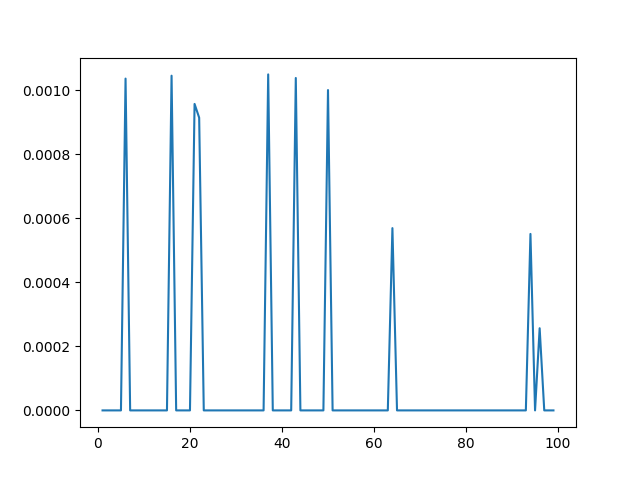
\includegraphics[scale = 0.7]{images/NN1fig2.png}
\end{center}

\subsection{Pairwise Exchange Method}

For the purpose of this analysis, the algorithm was made to run for 4 different instances of a graph with n vertices. In all 4 instances, the weights of the graph are randomly assigned while completeness of the graph is maintained. The average time of all 4 instances was taken to better gauge the performance of this algorithm. The algorithm is allowed to run until the total weight of the Hamiltonian path converges to an optimal value.

There are some $sharp$ fluctuations in the graph which are random and points to the differing rate of convergence of the total weight of hamiltonian paths passed into the algorithm as discussed in the theoretical analysis. 

\begin{center}
    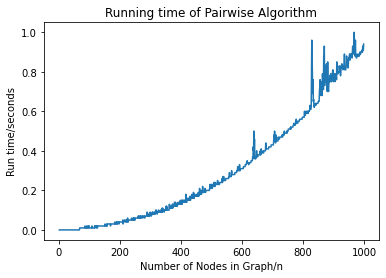
\includegraphics[scale = 0.75]{2_opt.png}
\end{center}

The following table reports the plotted values in the graph. It can be observed that the average run time has an accelerating rate of increase for every subsequent hundredth n. Therefore, the arbitrary paths have a slower convergence in total weight. However, due to low computational power, the algorithm could not be run for a sufficiently large number of nodes in order to observe a conclusive trend in the average run time.

\begin{center}
\begin{tabular}{ |c|c|c| } 
 \hline
 number of nodes/n & time/seconds \\ 
 \hline
 100 & 0.01  \\ 
 \hline
 200 & 0.04 \\ 
 \hline
 300 & 0.08 \\ 
 \hline
 400 & 0.13  \\ 
 \hline
 500 & 0.23 \\ 
 \hline
 600 & 0.31 \\ 
 \hline
 700 & 0.43  \\ 
 \hline
 800 & 0.57 \\ 
 \hline
 900 & 0.77 \\ 
 \hline
 999 & 0.94  \\ 
 \hline
\end{tabular}
\end{center}
     
\subsection {Christofides–Serdyukov Algorithm}

\begin{center}
    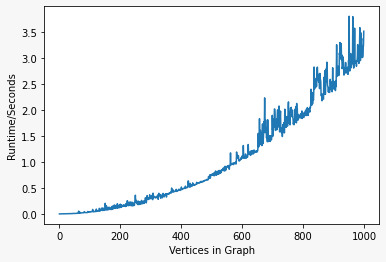
\includegraphics[scale = 0.75]{images/christ100.jpeg}
\end{center}
\begin{center}
\begin{tabular}{ |c|c|c| } 
 \hline
 number of nodes/n & time/seconds \\ 
 \hline
 100 & 0.03167510 \\ 
 \hline
 200 & 0.12088537 \\ 
 \hline
 300 & 0.36213731 \\ 
 \hline
 400 & 0.57751178  \\ 
 \hline
 500 & 0.81713914 \\ 
 \hline
 600 & 1.28897452 \\ 
 \hline
\end{tabular}
\end{center}
\vspace{3mm}
To analyze this algorithm, we ran it several times on graphs of different sizes 4 times, and then took an average value to plot. We can see that the algorithm is running in polynomial time. Specifically it can be seen through the graph that the algorithm runs in $O(n^3)$ time. It was difficult to run the graph on high values such as $n=1000$ for several times since it was too computationally expensive. Nevertheless, one can extrapolate the runtime of this algorithm with the plot.  
\chapter{Conclusion}

Since the traveling salesman problem is $\NP$-complete, finding an exact solution to a real-world problem is a futile task due to the computational constraints present. We saw the Held Karp algorithm in Chapter 1, which gave an exact solution but did so in exponential time. \\

On the other hand, approximate algorithms to the TSP provide a more realistic way to arrive at a solution. Although these solutions are not exact, they can be computed in reasonable times, given that the problem complies with certain conditions. The most accurate approximation algorithm for the TSP is the Christofides-Seryukov Algorithm, finding a solution with a 1.5 approximation ratio. \\

The TSP is a stellar example of compromising accuracy to achieve more practicality. There is still ongoing work on trying to find a more accurate approximation algorithm, the latest development being an even further reduction of the approximation ratio done in July 2020. Only time will tell how far we can go in finding a near-perfect solution to the TSP.  
\newpage
\chapter{References}
\begin{enumerate}
  \item Thomas H. Cormen, Charles E. Leiserson, Ronald L. Rivest, and Clifford Stein. 2009. Introduction to Algorithms, Third Edition (3rd. ed.)
  \paragraph{}

  \item David L. Applegate, Robert E. Bixby, Vasek Chvatal, and William J. Cook. 2007. The Traveling Salesman Problem: A Computational Study. Princeton University Press, USA
  \paragraph{}
  \item Hutchinson, Charles et al. CMU Traveling Salesman Problem. 2016, \url{https://www.math.cmu.edu/~af1p/Teaching/OR2/Projects/P58/OR2_Paper.pdf}. Accessed 7 Dec 2020.
  \paragraph{}
  \item Kizilates, Gozde, and Fidan Nuriyeva. On The Nearest Neighbor Algorithms For The Traveling Salesman Problem. 2013, \url{https://www.researchgate.net/publication/289195926_On_the_Nearest_Neighbor_Algorithms_for_the_Traveling_Salesman_Problem.} Accessed 7 Dec 2020.
  \paragraph{}
  \item Chapter 1: The Mathematics Of Voting. \url{http://www.math.hawaii.edu/~les/m100/lecture9.pdf} Accessed 7 Dec 2020.
\end{enumerate}
\newpage

\end{document}